%%%%%%%%%%%%%%%%%%%%%%%%%%%%%%%%%%%%%%%%%%  不使用 authblk 包制作标题  %%%%%%%%%%%%%%%%%%%%%%%%%%%%%%%%%%%%%%%%%%%%%%
%-------------------------------PPT Title-------------------------------------
\title{19-\rm{Berry}相位 多体相互作用理论}
%-----------------------------------------------------------------------------
%----------------------------Author & Date------------------------------------

%\author[\textrm{Jun\_Jiang}]{姜\;\;骏\inst{}} %[]{} (optional, use only with lots of authors)
%% - Give the names in the same order as the appear in the paper.
%% - Use the \inst{?} command only if the authors have different
%%   affiliation.
%\institute[BCC]{\inst{}%
\institute[Gain~Strong]{\inst{}%
%\vskip -20pt 北京市计算中心}
\vskip -20pt {\large 格致斯创~科技}}
\date[\today] % (optional, should be abbreviation of conference name)
{%	{\fontsize{6.2pt}{4.2pt}\selectfont{\textcolor{blue}{E-mail:~}\url{jiangjun@bcc.ac.cn}}}
\vskip 45 pt {\fontsize{8.2pt}{6.2pt}\selectfont{%清华大学\;\;物理系% 报告地点
	\vskip 5 pt \textrm{2023.04.22}}}
}

%% - Either use conference name or its abbreviation
%% - Not really information to the audience, more for people (including
%%   yourself) who are reading the slides onlin%%   yourself) who are reading the slides onlin%%   yourself) who are reading the slides onlineee
%%%%%%%%%%%%%%%%%%%%%%%%%%%%%%%%%%%%%%%%%%%%%%%%%%%%%%%%%%%%%%%%%%%%%%%%%%%%%%%%%%%%%%%%%%%%%%%%%%%%%%%%%%%%%%%%%%%%%

\subject{}
% This is only inserted into the PDF information catalog. Can be left
% out.
%\maketitle
\frame
{
%	\frametitle{\fontsize{9.5pt}{5.2pt}\selectfont{\textcolor{orange}{“高通量并发式材料计算算法与软件”年度检查}}}
\titlepage
}
%-----------------------------------------------------------------------------

%------------------------------------------------------------------------------列出全文 outline ---------------------------------------------------------------------------------
%\section*{}
%\frame[allowframebreaks]
%{
%  \frametitle{Outline}
%%  \frametitle{\textcolor{mycolor}{\secname}}
%  \tableofcontents%[current,currentsection,currentsubsection]
%}
%%在每个section之前列出全部Outline
%%类似的在每个subsection之前列出全部Outline是\AtBeginSubsection[]
%\AtBeginSection[]
%{
%  \frame<handout:0>%[allowframebreaks]
%  {
%    \frametitle{Outline}
%%全部Outline中,本部分加亮
%    \tableofcontents[current,currentsection]
%  }
%}

%-----------------------------------------------PPT main Body------------------------------------------------------------------------------------
\small
%\section{\rm{VASP~}软件中\rm{PAW~}计算的实现}
%\frame
%
%	\frametitle{\textrm{VASP}计算的特色}
%	相比于与普通的第一原理计算软件,\textrm{VASP}很好地平衡了计算效率和精度的问题,总的来说,\textrm{VASP}主要通过这几个特色保证了计算的高效能
%	\begin{itemize}
%	     \item 迭代与优化算法的多样性\\
%		     本质上电荷密度迭代 \textrm{\&\&} 体系总能量优化是相同的优化问题,采用了类似的算法\upcite{CMS6-15_1996,PRB54-11169_1996}:\\
%			\textcolor{blue}{\textrm{Pseudo-Newton、Conjugate-Gradient、Broyden~mix、damping-factor、RMM-DIIS}}
%	     \item 尽可能采用局域基(原子轨道基)函数:~\\
%		     \textcolor{blue}{\textrm{LREAL}}=\textcolor{red}{\textrm{.TRUE.}}\\
%			优化的投影函数也尽可能在实空间表示
%	     \item \textrm{PAW}原子数据集:\textcolor{blue}{优异的赝势}\upcite{PRB59-1758_1999}
%	\end{itemize}
%}
\section{极化与\rm{Berry~}相位}
\frame
{
	\frametitle{电介质材料的极化与\textrm{Berry~}相位}
	\textcolor{blue}{电极化}:~电介质内部正负电荷的相对位移,会产生电偶极子,这现象称为电极化
	\begin{itemize}
\setlength{\itemsep}{10pt}
		\item \textcolor{red}{压电效应}:~\textcolor{blue}{电介质沿一定方向受外力发生形变时,内部会产生极化现象:~在电解质两个相对表面出现正负相反电荷;当作用力方向改变时,电荷的极性也随之改变;当外力去掉后,又会恢复到不带电的状态}
		\item \textcolor{red}{热电效应}:~\textcolor{blue}{电介质因为受热,电子(空穴)由高温区往低温区移动时,产生电荷堆积引起极化}
		\item \textcolor{red}{铁电效应}:~\textcolor{blue}{某些电介质中,晶胞的结构使正负电荷中心不重合而出现电偶极矩,在内部产生非零的电极化强度,使晶体具有自发极化,且电偶极矩方向可以因外电场而改变,呈现出类似于铁磁体的特点}
	\end{itemize}
}

\frame
{
	\frametitle{外电场下的极化}
	\begin{itemize}
		\item 金属在外电场下的极化
\begin{figure}[h!]
\centering
%\hspace*{-10pt}
\vspace*{-0.15in}
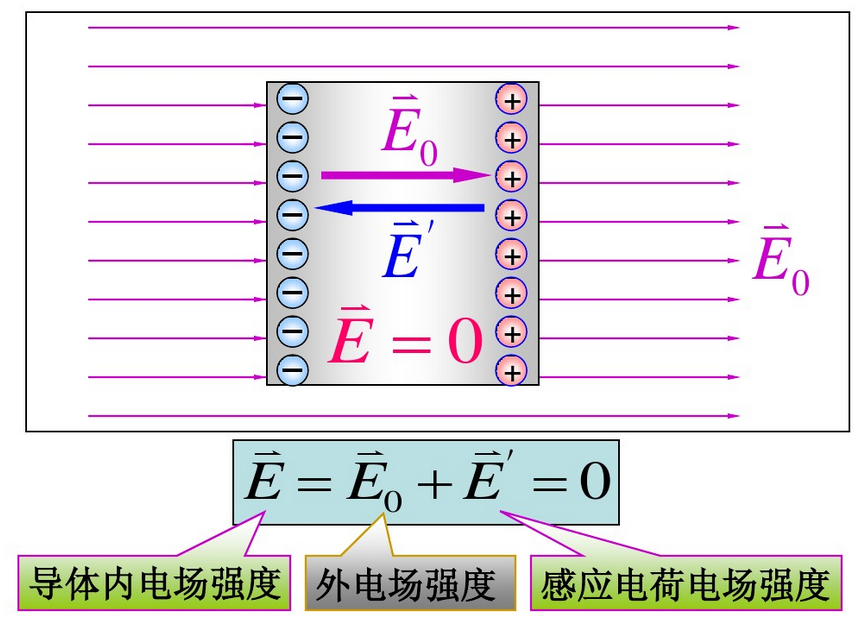
\includegraphics[height=1.8in,width=3.3in,viewport=0 0 1100 650,clip]{Figures/Polarize_metal-2.png}
\caption{\tiny \textrm{Schematic of a metal in the static electric field.}}%
\label{Polarization_metal}
\end{figure} 
\textcolor{blue}{金属体相的物理性质不会受外场的影响}
	\end{itemize}
}

\frame
{
	\frametitle{外电场下的极化}
	\begin{itemize}
		\item 绝缘体在外电场下的极化\\
			根据电磁理论,电场极化强度可定义为
			\begin{displaymath}
				\nabla\cdot\vec P(\vec r,t)=-\delta n(\vec r,t)
			\end{displaymath}
			利用极化电流守恒条件$\nabla\cdot\mathbf{j}(\vec r,t)=-\mathrm{d}n(\vec r,t)/\mathrm{d}t$\\
			可得电场极化强度与极化电流密度关系
			\begin{displaymath}
				\frac{\mathrm{d}\vec P(\vec r,t)}{\mathrm{d}t}=\mathbf{j}(\vec r,t)+\nabla\times\mathbf{M}(\vec r,t)
			\end{displaymath}
			这里$\mathbf{M}(\vec r,t)$是任意矢量场

			宏观电场极化强度一般定义为:\\\textcolor{blue}{单位体积中分子电偶极矩的矢量和}
	\end{itemize}
	\textcolor{red}{这样定义的极化强度存在一定的问题}
}

\frame
{
	\frametitle{外电场下的极化}
			\begin{enumerate}
				\item 对于有限体系,上述定义的电场极化强度是合理的
\begin{figure}[h!]
\centering
%\hspace*{-10pt}
\vspace*{-0.15in}
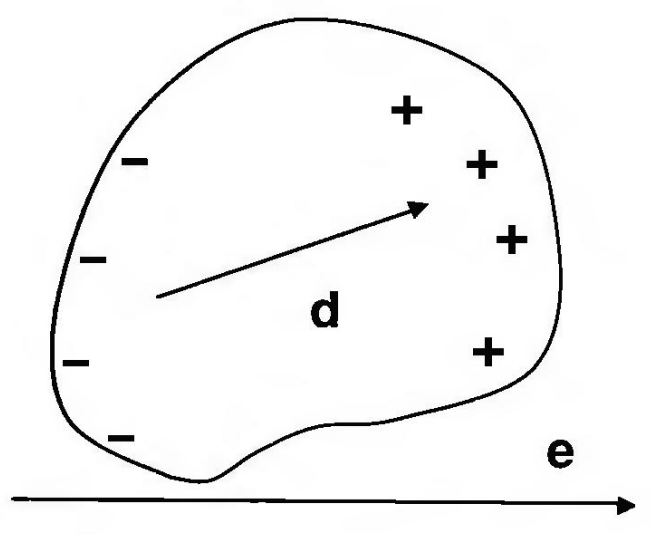
\includegraphics[height=0.9in,width=2.2in,viewport=0 0 1100 550,clip]{Figures/Polarize_insulator.png}
\caption{\tiny \textrm{Illustration of finite system for which the total dipole moment is well defined.}}%
\label{Polarization_insulator}
\end{figure} 
考虑到有限体系外$\vec P(\vec r)=0$,宏观电场极化强度$\vec P$可用偶极矩$\vec d$表示
\begin{displaymath}
	\vec P\equiv\frac{\vec d}{\Omega}=\frac1{\Omega}\int_{\mathrm{all\;space}}\mathrm{d}\vec rn(\vec r)\vec r
\end{displaymath}
\textcolor{red}{电场极化强度的变化$\Delta\vec P=\vec P^{(1)}-\vec P^{(0)}$只与电荷密度的改变$\Delta n=n^{(1)}-n^{(0)}$有关,而与电荷密度改变的路径有关}
			\end{enumerate}
}

\frame
{
	\frametitle{}
			\begin{enumerate}
				\setcounter{enumi}{1}
				\item 对于周期体系
\begin{figure}[h!]
\centering
%\hspace*{-10pt}
\vspace*{-0.15in}
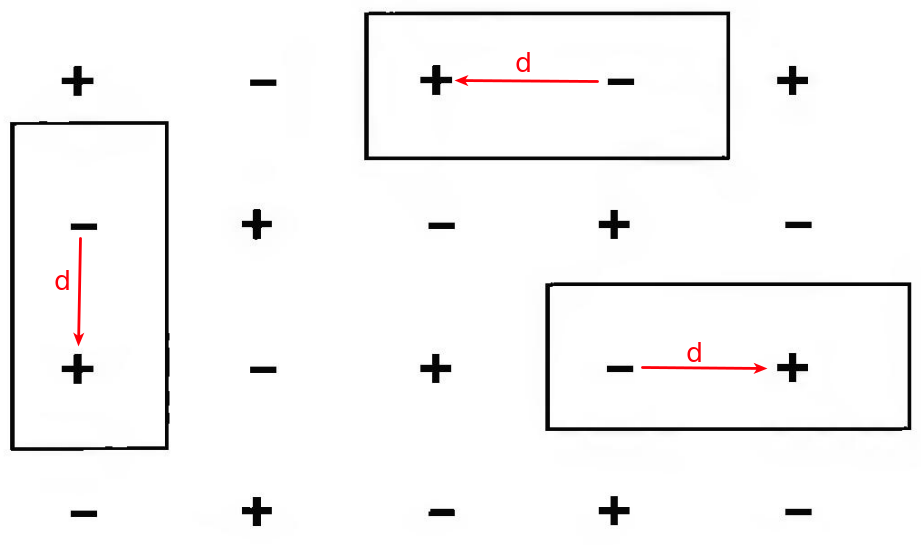
\includegraphics[height=0.9in,width=1.6in,viewport=0 0 1100 540,clip]{Figures/Polarize_insulator-2.png}
\caption{\textrm{\fontsize{7.5pt}{5.2pt}\selectfont{Point charge model of an ionic crystal. The dipole is obviously not unique since the cells shown all have different moments.}}}%
\label{Polarization_insulator-2}
\end{figure} 
正确定义周期体系的宏观电场极化强度,\textcolor{red}{必须用合适的形式代替对$\vec r$的无限积分}\\
宏观极化电流是极化过程中唯一可观测的物理量,极化强度的变化$\vec P$可由体相极化电流计算
\begin{displaymath}
	\vec P(\vec r,t)=\int^t\mathrm{d}t^{\prime}\mathbf{j}_{\mathrm{int}}(\vec r,t^{\prime})
\end{displaymath}
			\end{enumerate}
}

\frame
{
	\frametitle{现代极化理论与几何\textrm{Berry~}相位}
	\begin{itemize}
		\item 用极化电流计算电场极化定义虽然正确,但不能证明电场极化强度与积分路径无关
		\item \textrm{King-Smith}和\textrm{Vanderbilt}提出了新的计算方案%\upcite{PRB47-1651_1993}
			:\\
		\textcolor{red}{基本假设}:~连续的绝热变化可关联\textrm{Kohn-Sham}方程的\textrm{Hamiltonian}描述的不同态\\如果满足条件
	\begin{enumerate}
		\item 没有任何外部电场存在 
		\item 体系始终保持绝缘体状态
	\end{enumerate}
	宏观电场极化极化强度的变化可表示为
	\begin{displaymath}
		\Delta\vec P=\int_0^1\mathrm{d}\lambda\frac{\partial\vec P}{\partial\lambda}
	\end{displaymath}
	\textcolor{red}{注意}:~对所有的$\lambda$,宏观外电场要求为0
	\end{itemize}
}

\frame
{
	\frametitle{现代极化理论与几何\textrm{Berry~}相位}
	\begin{itemize}
		\item 根据线性响应理论,\textrm{Resta}指出:~在无限体系中,微扰项$\partial\vec P/\partial\lambda$可以用动量矩阵元表示%\upcite{RMP66-899_1994}
	\begin{displaymath}
		\frac{\partial\vec P}{\partial\lambda}=-\mathrm{i}\frac{\mathrm{e}\hbar}{\Omega m_e}\sum_{\vec k}\sum_i^{\mathrm{occ}}\sum_j^{\mathrm{empty}}\frac{\langle\psi_{\vec k i}^{\lambda}|\hat{\vec p}|\psi_{\vec k j}^{\lambda}\rangle\langle\psi_{\vec k i}^{\lambda}|\partial V_{\mathrm{KS}}^{\lambda}/\partial\lambda|\psi_{\vec k j}^{\lambda}\rangle}{(\varepsilon_{\vec k i}^{\lambda}-\varepsilon_{\vec k j}^{\lambda})^2}+\mathrm{c.c.}
	\end{displaymath}
	这里对$i,j$的求和遍历所有自旋态
	\item 早先\textrm{Thouless}等在讨论量子\textrm{Hall~}效应时曾证明,上述对所有态的求和可变换成只对占据态的求和%\upcite{PRL49-405_1982}
		\\引入与$\vec k$有关的\textrm{Kohn-Sham~}势$V_{\mathrm{KS}}^{(\lambda)}(\vec r)$,因此周期性\textrm{Hamiltonian~}表示为
	\begin{displaymath}
		\hat H(\vec k,\lambda)=\frac1{2m_e}\left( -\mathrm{i}\hbar\nabla+\hbar\vec k \right)^2+V_{\mathrm{KS}}^{(\lambda)}(\vec r)
	\end{displaymath}
	\end{itemize}
}

\frame
{
	\frametitle{现代极化理论与几何\textrm{Berry~}相位}
	利用\textrm{Bloch~}函数
	\begin{displaymath}
		\psi_{\vec k i}^{\lambda}=\mathrm{e}^{\mathrm{i}\vec k\cdot\vec r}u_{\vec k i}^{\lambda}(\vec r)
	\end{displaymath}
	满足等式
	\begin{displaymath}
		\hat H(\vec k,\lambda)u_{\vec k i}^{\lambda}(\vec r)=\left[ -\frac{\hbar}{2m_e}(\nabla+\mathrm{i}\vec k)^2 +V_{\mathrm{KS}}^{(\lambda)}(\vec r)\right]u_{\vec k i}^{\lambda}(\vec r)=\varepsilon_{\vec k i}^{\lambda}u_{\vec k i}^{\lambda}(\vec r)
	\end{displaymath}
	根据\textcolor{red}{对易关系}
	\begin{displaymath}
		\langle\psi_{\vec k i}^{\lambda}|\hat{\vec p}|\psi_{\vec k j}^{\lambda}\rangle=\frac{m_e}{\hbar}\langle u_{\vec k i}^{\lambda}|[\partial/\partial\vec k,\hat H(\vec k,\lambda)]|u_{\vec k j}^{\lambda}\rangle
	\end{displaymath}
	\begin{displaymath}
		\langle\psi_{\vec k i}^{\lambda}|\partial V_{\mathrm{KS}}^{\lambda}/\partial\lambda|\psi_{\vec k j}^{\lambda}\rangle=\frac{m_e}{\hbar}\langle u_{\vec k i}^{\lambda}|[\partial/\partial\lambda,\hat H(\vec k,\lambda)]|u_{\vec k j}^{\lambda}\rangle
	\end{displaymath}
	可得
	\begin{displaymath}
		\Delta\vec P_{\alpha}=-|e|\frac2{(2\pi)^3}\mathrm{Im}\int_{\mathrm{BZ}}\mathrm{d}\vec k\int_0^1\mathrm{d}\lambda\sum_i^{\mathrm{occ}}\left\langle\frac{\partial u_{\vec k i}^{(\lambda)}}{\partial k_{\alpha}}\right|\left.\frac{\partial u_{\vec k j}^{(\lambda)}}{\partial\lambda}\right\rangle
	\end{displaymath}
	对$\vec k$~的积分是倒空间的第一\textrm{Brillouin zone}
}

\frame
{
	\frametitle{现代极化理论和几何\textrm{Berry~}相位}
	\textrm{Thouless~}在讨论无相互作用粒子的量子\textrm{Hall~}效应时曾给出类似的积分表达式%\upcite{PRB27-6083_1983}
	,利用\textrm{Stokes~}定律
\begin{figure}[h!]
\centering
%\hspace*{-10pt}
\vspace*{-0.12in}
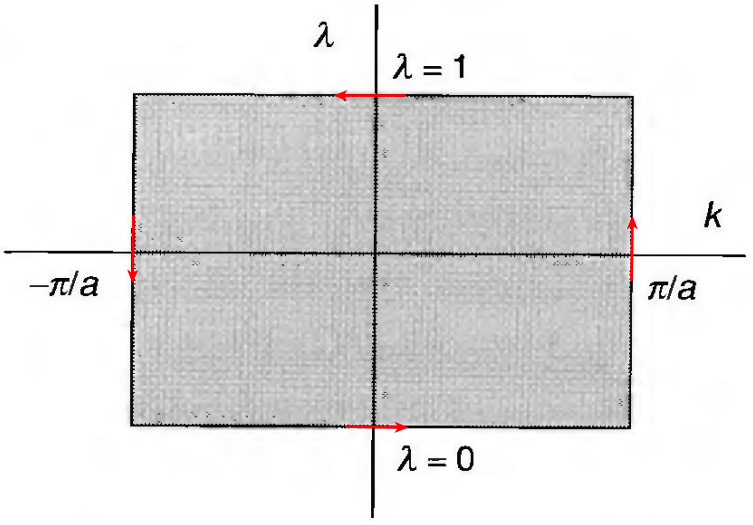
\includegraphics[height=1.2in,width=1.6in,viewport=0 0 800 540,clip]{Figures/Berry_contour_integration.png}
\caption{\tiny \textrm{Schematic figure of region of integration in $(k,\lambda)$ space for calculation of $\Delta P$ using the contour of integration C.}}%
\label{Berry_contour_integration}
\end{figure} 
	\begin{displaymath}
		\Delta P=-|e|\frac2{(2\pi)^3}\mathrm{Im}\sum_i^{\mathrm{occ}}\left\{ \underline{\textcolor{blue}{\oint_C\sum_{j=1}^2\mathrm{d}\tau_j\langle u_{k i}^{\lambda}|\partial/\partial\tau_j|u_{k i}^{\lambda}\rangle}} \right\} 
	\end{displaymath}
这里$\tau$~是二维空间$(\lambda,k)$,$C$是$\tau$空间的围道
}

\frame
{
	\frametitle{现代极化理论和几何\textrm{Berry~}相位}
	\begin{itemize}
		\item 上述大括号内的积分是\textcolor{red}{绝热近似下,利用周期波函数围道积分计算的\textrm{Berry~}相位改变}%\upcite{PRS392-45_1984,PRL51-2167_1983}
		\item \textrm{Thouless~}指出上述围道积分对应的是在势$V_{\mathrm{KS}}^{(0)}=V_{\mathrm{KS}}^{(1)}$条件下的积分,\textcolor{blue}{围道积分计算的是实空间波函数点的相位变化}
		\item 考虑到波函数的周期性,用$(k,\lambda)$表示的相位变化可以加$2n\pi$而不变
	\end{itemize}
	利用周期函数$u_{\vec k i}^{(\lambda)}$的“周期标度关系”
	\begin{displaymath}
		u_{\vec k+\vec G i}^{(\lambda)}(\vec r)=\textcolor{green}{\mathrm{e}^{\mathrm{i}\vec G\cdot\vec r}}u_{\vec k i}^{(\lambda)}(\vec r)
	\end{displaymath}
	其中$\vec G$是倒空间格矢,因此这种标度关系并不唯一
%	选择$\vec G$满足在$\vec k$和$\vec k+\vec G$对$\lambda$的二重积分相互抵消,因此
	\begin{displaymath}
		\Delta\vec P_{\alpha}=\mathrm{i}\frac{-|e|}{(2\pi)^3}\sum_i^{\mathrm{occ}}\int_{\mathrm{BZ}}\mathrm{d}\vec k\left[ \langle u_{\vec k i}^{\lambda=1}|\partial/\partial_{k_{\alpha}}|u_{\vec k i}^{\lambda=1}\rangle-\langle u_{\vec k i}^{\lambda=0}|\partial/\partial_{k_{\alpha}}|u_{\vec k i}^{\lambda=0}\rangle \right]
	\end{displaymath}
}

\frame
{
	\frametitle{现代极化理论和几何\textrm{Berry~}相位}
	利用周期标度关系,可有
	\begin{displaymath}
		\Delta\vec P=\vec P^{(1)}-\vec P^{(0)}	
	\end{displaymath}
	其中
	\begin{displaymath}
		P_{\alpha}^{(\lambda)}=\mathrm{i}\frac{-|e|}{(2\pi)^3}\sum_i^{\mathrm{occ}}\int_{\mathrm{BZ}}\mathrm{d}\vec k\langle u_{\vec k i}^{(\lambda)}|\partial/\partial_{k_{\alpha}}|u_{\vec k i}^{(\lambda)}\rangle
	\end{displaymath}
	\textrm{Zak~}等指出,\textcolor{red}{上述表达式即能带$i$的\textrm{Berry~}相位}%\upcite{PRL62-2747_1989,EPL18-239_1992}
	
	\textcolor{blue}{注意到\textrm{Wannier~}函数的形式与“周期标度”的相位密切相关},有
	\begin{displaymath}
		u_{\vec k i}^{(\lambda)}(\vec r)=\frac 1{\sqrt N}\sum_{\vec R}\mathrm{e}^{-\mathrm{i}\vec k\cdot(\vec r-\vec R)}w_i^{(\lambda)}(\vec r-\vec R)
	\end{displaymath}
	利用\textrm{Wannier~}函数,$P_{\alpha}^{(\lambda)}$可以具有更简单的形式
	\begin{displaymath}
		\vec P^{(\lambda)}=-\frac{2e}{\Omega}\sum_i^{\mathrm{occ}}\int\vec r|w_i^{(\lambda)}(\vec r)|^2\mathrm{d}\vec r
	\end{displaymath}
	这里$\Omega$是原胞体积
}

\frame
{
	\frametitle{现代极化理论和几何\textrm{Berry~}相位}
	\textcolor{red}{电介质的极化改变正比于由绝热变化引起的\textrm{Wannier~}函数的电荷中心的偏移}

	考虑到绝热变化要求$V_{\mathrm{KS}}^{(0)}=V_{\mathrm{KS}}^{(1)}$,因此周期函数$u_{\vec k i}^{(0)}$和$u_{\vec k i}^{(1)}$仅有相位的差别
	\begin{displaymath}
		u_{\vec k i}^{(1)}=\mathrm{e}^{\mathrm{i}\theta_{\vec k i}}u_{\vec k i}^{(\lambda)}
	\end{displaymath}
	因此
	\begin{displaymath}
		\Delta P_{\alpha}=-\frac{|e|}{(2\pi)^3}\sum_i^{\mathrm{occ}}\int_{\mathrm{BZ}}\mathrm{d}\vec k\partial\theta_{\vec k i}/\partial k_{\alpha}
	\end{displaymath}
	$\mathrm{e}^{\mathrm{i}\theta_{\vec k i}}$是$\vec k$的周期函数,最一般的相位表示$\theta_{\vec k i}=\beta_{\vec k i}+\vec k\cdot\vec R$,因此
	\begin{displaymath}
		\Delta\vec P=-\frac{2e}{\Omega}\sum_i^{\mathrm{occ}}\vec R_i
	\end{displaymath}
}

\frame
{
	\frametitle{现代极化理论和几何\textrm{Berry~}相位}
	\begin{itemize}
		\item \textcolor{blue}{原胞内极化强度的变化即$-(2e/\Omega)R$}
		\item 特别地,考虑由于晶格平移$V_{\mathrm{KS}^{(\lambda)}}(\vec r)=V_{\mathrm{KS}}^{(0)}(\vec r-\lambda\vec R)$\\
			引起极化$\Delta P$为
			\begin{displaymath}
				\Delta P=-\frac{2e}{\Omega}N_{\mathrm{occ}}\vec R
			\end{displaymath}
	\end{itemize}
	实际计算$\Delta\vec P$有一定的复杂性:~\textcolor{blue}{因为\textrm{Brillouin zone}有限$\vec k$点上的本征态\textrm{Blochl~}函数间没有相关系}\\
	为了回避此困难,采用以下策略
	\begin{itemize}
		\item 选定格矢$\vec G_{\lVert}$平行于倒空间原胞最短的格矢,沿该方向
			\begin{displaymath}
				\Delta P_{\lVert}=P_{\lVert}^{(1)}-P_{\lVert}^{(0)}
			\end{displaymath}
			并有
			\begin{displaymath}
				P_{\lVert}^{(\lambda)}=\mathrm{i}\frac{-|e|}{(2\pi)^3}\int_{\mathrm{A}}\mathrm{d}\vec k_{\bot}\sum_i^{\mathrm{occ}}\int_0^{|\vec G_{\lVert}|}\mathrm{d}k_{\lVert}\left\langle u_{\vec k i}^{(\lambda)}\right|\frac{\partial}{\partial k_{\lVert}}\left|u_{\vec k i}^{(\lambda)}\right\rangle
			\end{displaymath}

	\end{itemize}
}

\frame
{
	\frametitle{现代极化理论和几何\textrm{Berry~}相位}
	\begin{itemize}
		\item 为完成积分,$\vec k$~空间的布点离散方案设置如下
			\begin{enumerate}
				\item 垂直于$\vec G_{\lVert}$方向的2\textrm{D~}平面上,采用传统的\textrm{Monkhorst-Pack}布点
				\item 在$\vec k_{\lVert}$方向上离散$J$个$\vec k$点
\begin{displaymath}
	\vec k_j=\vec k_{\bot}+j\vec G_{\lVert}/J
\end{displaymath}
这里$j$的取值由0到$J-1$\\
由此得到
\begin{equation}
	\phi_J^{(\lambda)}(\vec k_{\bot})=\mathrm{Im}\left\{ \ln\prod_{j=0}^{J-1}\det(\langle u_{\vec k_j m}^{(\lambda)}|u_{\vec k_{j+1 n}}^{(\lambda)}\rangle) \right\}
	\label{eq:phase_angle}
\end{equation}
这里$u_{\vec k_J n}^{(\lambda)}=\mathrm{e}^{-\mathrm{i}\vec G_{\lVert}\cdot\vec r}u_{\vec k_0 n}^{(\lambda)}$\\
$n$和$m$遍历全部电子占据的价带
			\end{enumerate}
	\end{itemize}
}

\frame
{
	\frametitle{现代极化理论和几何\textrm{Berry~}相位}
	在$J\rightarrow\infty$极限条件下
	\begin{displaymath}
		\begin{aligned}
			\phi^{(\lambda)}(\vec k_{\bot})\equiv&\lim_{J\rightarrow\infty}\phi_J^{(\lambda)}(\vec k_{\bot})\\
			&=-\mathrm{i}\sum_{i}^{\mathrm{occ}}\int_0^{|G_{\lVert}|}\mathrm{d}k_{\lVert}\langle u_{\vec k i}^{(\lambda)}|\partial/\partial k_{\lVert}|u_{\vec k i}^{(\lambda)}\rangle
		\end{aligned}
	\end{displaymath}
	于是$P_{\lVert}^{(\lambda)}$可表示为
	\begin{displaymath}
		P_{\lVert}^{(\lambda)}=\mathrm{i}\frac{2|e|}{(2\pi)^3}\int_{\mathrm A}\mathrm{d}\vec k_{\bot}\phi^{\lambda}(\vec k_{\bot})
	\end{displaymath}
	由此可知式\eqref{eq:phase_angle}中波函数的乘积与相位选择无关:\\
	\textcolor{blue}{$u_{\vec k i}^{(\lambda)}$的相位改变}\textcolor{red}{引起$P_{\lVert}^{(\lambda)}$的相位角上增加改变$n\cdot2\pi$}
}

%\section{匀强电场下的电介质与\rm{Berry~}相位}
\frame
{
	\frametitle{匀强电场下的电介质}
	\begin{itemize}
		\item \textcolor{purple}{极化与波函数相位的关系深化了对密度泛函理论的基态密度与周期体系物性的认识}
		\item 为处理介质处于匀强电场下的问题,\textrm{Nunes}和\textrm{Gonze}发展出了结合现代极化理论和变分-微扰(\textrm{variation-perturbation})的计算方法%\upcite{PRB63-155107_2001}
			\begin{enumerate}
				\item 将外加匀强电场作为微扰
				\item 假设微扰极化的占据能带仍可用\textrm{Berry~}相理论表示\\
					\textcolor{blue}{外加匀强电场虽然破坏了体系平移周期性,电荷密度仍保持体系周期性,\textrm{Berry~}相位由极化的周期波函数计算}
				\item 波函数用微扰展开到二阶或更高,用变分迭代计算介电响应函数
			\end{enumerate}
		\item 将\textrm{Berry~}相位用电子波函数级数展开,必须要作离散化\\
			\begin{enumerate}
				\item \textrm{DAPE}:~先对\textrm{Hamiltonian}作微扰推导,再离散化计算\textrm{Berry~}相位
				\item \textrm{PEAD}:~在场相关\textrm{Hamiltonian~}基础上先离散计算\textrm{Berry~}相位,再作微扰推导
			\end{enumerate}
	\end{itemize}
}

\section{电子相关与多体理论}
\frame
{
	\frametitle{\textrm{Green function}}
	\begin{itemize}
		\item 时间序列的\textrm{Green's function}定义为$G(\vec r_1,t_1;\vec r_2,t_2)=-\mathrm{i}\langle\Theta_0^N|\hat{\mathbf{T}}[\hat\psi(\vec r_1,t_1)\hat\psi^{\dag}(\vec r_2,t_2)]|\Theta_0^N\rangle$
		\item \textrm{Green function}的\textrm{Lehmann}表象为$$G(\vec r_1,\vec r_2;\omega)=\sum\limits_i\dfrac{\Psi_i(\vec r_1)\Psi_i^{\dag}(\vec r_2)}{\omega-\varepsilon_i+\mathrm{i}\eta\mathrm{sign}(\varepsilon_i-\mu)}\qquad\eta\rightarrow0^+$$
			由于频率域中时间序列的\textrm{Green's function}包含$(N-1)$个粒子和$(N+1)$个粒子体系的全部激发谱,它们与\textrm{Green's function}在复平面的极值对应
	\end{itemize}
\begin{figure}[h!]
\centering
\vspace{-5pt}
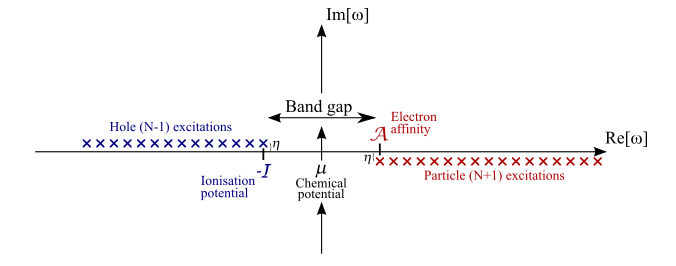
\includegraphics[height=0.80in,width=2.05in,viewport=30 1 660 265,clip]{Figures/GW-0.png}
\caption{\textrm{\small{The poles of the time-ordered Green's function.}}}%(与文献\cite{EPJB33-47_2003}图1对比)
\label{GW-0}
\end{figure}
}

\frame
{
	\frametitle{多重散射与\textrm{Green's function}}
\begin{figure}[h!]
\centering
	\vspace{-20pt}
%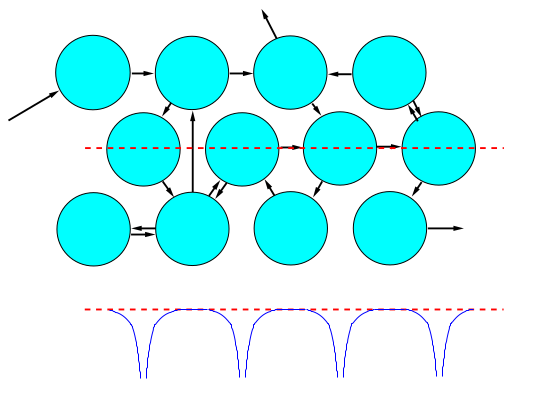
\includegraphics[height=1.80in,width=1.95in,viewport=5 0 515 495,clip]{Figures/multiple-scattering_theory.png}
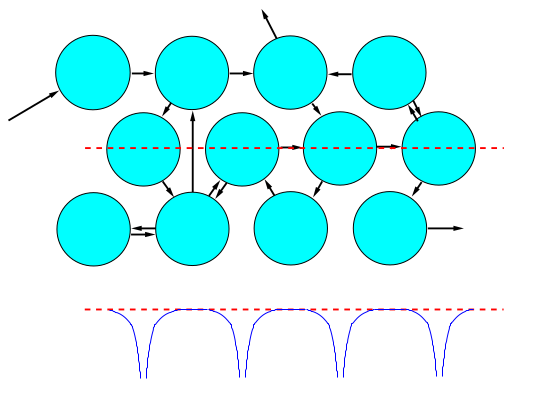
\includegraphics[height=2.50in,width=2.64in,viewport=5 0 515 495,clip]{Figures/multiple-scattering_theory.png}
\caption{\tiny \textrm{Central idea of multiple scattering theory:~ decomposition of electronic motion into scattering at atomic sites and free-electron like propagation in between. The bottom of the figure gives a sketch for the potential along the dashed line.}}
\label{Multi-scattering}
\end{figure}
}

\frame
{
	\frametitle{多重散射与\textrm{Green's function}}
\begin{figure}[h!]
	\vspace{-5pt}
\centering
\animategraphics[autoplay, loop, height=1.2in]{1}{Figures/Multi_scattering-}{0}{9}
\label{Multiple_scattering-0-9}
\end{figure}
\textcolor{blue}{多重散射:~}入射波是\textcolor{red}{所有来自其他散射中心的出射波叠加}
			\begin{displaymath}
				\begin{aligned}
					\tilde G=&\tilde G_0+G_0\mathbf{t}\tilde G_0+G_0\mathbf{t}\tilde G_0\mathbf{t}\tilde G_0+\cdots\\
					=&\tilde G_0+\tilde G_0\mathbf{t}\tilde G \Longrightarrow \tilde G=(\tilde G_0^{-1}-\mathbf{t})^{-1}
%					\tilde G=&(\tilde G_0^{-1}-\mathbf{t})^{-1}
				\end{aligned}
			\end{displaymath}
}

\frame
{
	\frametitle{\textrm{Green function}与自能}
	\textrm{Dyson}方程
	\begin{displaymath}
		\begin{aligned}
	&G(\vec r_1,t_1;\vec r_2,t_2)=G_0(\vec r_1,t_1;\vec r_2,t_2)\\
	&+\int G_0(\vec r_1,t_1;\vec r_3,t_3)\Sigma(\vec r_3,t_3;\vec r_4,t_4)G(\vec r_4,t_4;\vec r_2,t_2)\mathrm{d}t_3\mathrm{d}\vec r_3\mathrm{d}t_4\mathrm{d}\vec r_4
		\end{aligned}
	\end{displaymath}
	\begin{itemize}
		\item \textrm{Dyson}方程描述了相互作用体系$G$通过自能$\Sigma$与近独立体系(传播子)$G_0$关联,自能$\Sigma$是非局域,非\textrm{Hermitian},并与时间相关
		\item 通过求解含有自能$\Sigma$的准粒子方程,可以求解得到多体体系中重整化电子的量子态(\textrm{Hedin}方程)
			$$\bigg[\hat h_0(\vec r_1)+v_H(\vec r_1)\bigg]\Psi(\vec r_1)+\int\Sigma(\vec r_1,\vec r_2;\omega^{\mathrm{QP}})\Psi(\vec r_2)\mathrm{d}\vec r_2=\varepsilon^{\mathrm{QP}}\Psi(\vec r_1)$$
	\end{itemize}
}

\frame
{
	\frametitle{\textrm{Hedin}方程的求解} 
	\textrm{Hedin}方程是积分-微分,可以通过迭代求解
\begin{figure}[h!]
\centering
\vspace{-10pt}
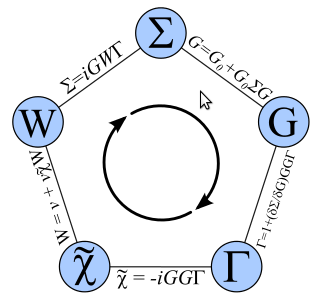
\includegraphics[height=1.0in,width=1.05in,viewport=5 5 330 335,clip]{Figures/GW-1.png}
%\caption{\textrm{\small{The relation of the varibous Green's function.}}}%(与文献\cite{EPJB33-47_2003}图1对比)
\label{GW-1}
\end{figure}
	\begin{itemize}
			\vspace{-15pt}
		\item 定义不可约极化率$\tilde\chi$,$\tilde\chi(\vec r_1,t_1;\vec r_2,t_2)\equiv\dfrac{\delta n(\vec r_1,t_1)}{\delta U_{e\!f\!f}(\vec r_2,t_2)}=-\mathrm{i}\dfrac{\delta G(\vec r_1,t_1,\vec r_1,t_1+\eta)_{\eta\rightarrow0}}{\delta U_{e\!f\!f}(\vec r_2,t_2)}$
		\item 定义动态屏蔽相互作用$W(\vec r_1,t_1;\vec r_2,t_2)\equiv\int\epsilon^{-1}(\vec r_1,t_1;\vec r_3,t_3)v(\vec r_3,r_3;\vec r_2,t_2)\mathrm{d}t_3\mathrm{d}\vec r_3$
		\item 介电矩阵与不可约极化率满足关系:
			\begin{displaymath}
				\begin{aligned}
					&\epsilon(\vec r_1,t_1;\vec r_2,t_2)\\
					=&\delta(\vec r_1,t_1;\vec r_2,t_2)-\int v(\vec r_,t_1,\vec r_3,t_3)\tilde\chi(\vec r_3,t_3;\vec r_2,t_2)\mathrm{d}t_3\mathrm{d}\vec r_3
				\end{aligned}
			\end{displaymath}
	\end{itemize}

}

\frame
{
	\frametitle{$GW$近似}
	直接求解\textrm{Hedin}方程是非常复杂的,有必要采取近似(把\textrm{vertex}函数用局域瞬时函数替代),这就是$GW$近似
	$$\Gamma(\vec r_{12},t_{12};\vec r_3t_3)\approx\delta(\vec r_1,t_1;\vec r_2,t_2)\delta(\vec r_1,t_1;\vec r_3,t_3)\equiv\Gamma^{GW}(\vec r_{12},t_{12};\vec r_3,r_3)$$
\begin{figure}[h!]
\centering
\vspace{-15pt}
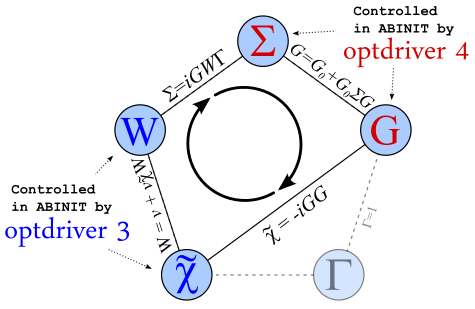
\includegraphics[height=1.0in,width=1.65in,viewport=5 5 530 320,clip]{Figures/GW-3.png}
%\caption{\textrm{\small{The relation of the varibous Green's function.}}}%(与文献\cite{EPJB33-47_2003}图1对比)
\label{GW-2}
\end{figure}
频率空间内,$GW$近似的自能表示为
$$\Sigma(\vec r_1,\vec r_2;\omega)=\dfrac{\mathrm i}{2\pi}\int \mathrm e^{\mathrm i\omega^{\prime}\delta^+}G(\vec r_1,\vec r_2;\omega+\omega^{\prime})W(\vec r_1,\vec r_2;\omega^{\prime})\mathrm{d}\omega^{\prime}$$
}

\frame
{
	\frametitle{由$GW$到$G_0W_0$近似}
	自洽迭代的$GW$方程求解仍然非常复杂,通常选择足够好的近似的$G$和$W$,作单次计算(即$G_0W_0$近似)得到自能
	$$\Sigma(\vec r_1,t_1;\vec r_2,t_2)=\mathrm{i}G_0^{\mathrm{KS}}W_0(\vec r_1,t_1+\eta;\vec r_2,t_2)_{\eta\rightarrow0}$$
	这里$G_0^{\mathrm{KS}}$由独立粒子的\textrm{Kohn-Sham(KS)}Hamiltonian

	屏蔽相互作用由\textrm{KS}本征态能量和波函数的\textrm{RPA}计算的到
	$$\chi^0(\vec r_1,t_1;\vec r_2,t_2)=-\mathrm{i}G_0^{\mathrm{KS}}(\vec r_1,t_1;\vec r_2,t_2)G_0^{\mathrm{KS}}(\vec r_1,t_1;\vec r_2,t_2)$$
	当准粒子波函数用\textrm{KS}轨道近似,本征态$\varepsilon^{\mathrm{KS}}$附近的准粒子能量$\varepsilon^{\mathrm{QP}}$用自能展开
	$$\varepsilon^{\mathrm{QP}}=\varepsilon^{\mathrm{KS}}+Z\langle\Psi^{\mathrm{KS}}|\Sigma(\varepsilon^{\mathrm{KS}}-v_{\mathrm{XC}})|\Psi^{\mathrm{KS}}\rangle$$
	这里重整化因子$Z$定义为$$Z\equiv\bigg[1-\langle\Psi^{\mathrm{KS}}\bigg|\dfrac{\partial\Sigma(\varepsilon)}{\partial\varepsilon^{\mathrm{KS}}}\bigg|\Psi^{\mathrm{KS}}\rangle\bigg]^{-1}$$
}

\frame
{
	\frametitle{$GWA$与\textrm{LDA+}$U$}
	\begin{displaymath}
		\begin{aligned}
			V_{m\sigma}^{GWA}=&\sum_{m^{\prime}\sigma^{\prime}}U_{mm^{\prime}}^0n_{m^{\prime}\sigma^{\prime}}-U_{mm}^0n_{m\sigma}-\sum_{m^{\prime}\neq m}J_{mm^{\prime}}n_{m^{\prime}\sigma}\\
			+&\left( \frac12-n_{m\sigma} \right)\sum_{m^{\prime}}W_{mm^{\prime}}
		\end{aligned}
	\end{displaymath}
	其中$U_{mm^{\prime}}^0$是\textcolor{blue}{未屏蔽\textrm{Coulomb~}相互作用矩阵},$J_{mm^{\prime}}$是\textcolor{blue}{交换矩阵}\\
	$W_{mm^{\prime}}$是\textcolor{red}{电子相关作用的矩阵$W_{\mathrm c}(\vec r,\vec r^{\prime};0)$的矩阵元}

	定义屏蔽相互作用参数$W$
	\begin{displaymath}
		W=-\sum_{m^{\prime}}W_{mm^{\prime}}
	\end{displaymath}
	因此,$\mathrm{GWA}$近似的矩阵元表示为
	\begin{displaymath}
			V_{m\sigma}^{GWA}=\sum_{m^{\prime}\sigma^{\prime}}U_{mm^{\prime}}^0n_{m^{\prime}\sigma^{\prime}}-(U_{mm}^0-W)n_{m\sigma}-\sum_{m^{\prime}\neq m}J_{mm^{\prime}}n_{m^{\prime}\sigma}-\frac12W
	\end{displaymath}
}

\frame
{
	\frametitle{$GWA$与\textrm{LDA+}$U$}
	对应于\textrm{LSDA},势能的修正
	\begin{displaymath}
		\begin{aligned}
			\delta V_{m\sigma}=&V_{m\sigma}^{GWA}-V_{m\sigma}^{\mathrm{LSDA}}\\
			=&\sum_{m^{\prime}\sigma^{\prime}}U_{mm^{\prime}}^0n_{m^{\prime}\sigma^{\prime}}-(U_{mm^{\prime}}^0-W)n_{m\sigma}-\sum_{m^{\prime}\neq m}J_{mm^{\prime}}n_{m^{\prime}\sigma}-\frac12W\\
			-&F^0\sum_{m^{\prime}\sigma^{\prime}}n_{m^{\prime}\sigma^{\prime}}+J\sum_mn_{m\sigma}+\frac12(F^0-J)\\
			=&\sum_{m^{\prime}\sigma^{\prime}}(U_{mm^{\prime}}^0-F^0)n_{m^{\prime}\sigma^{\prime}}-(U_{mm^{\prime}}^0-W)n_{m\sigma}-\sum_{m^{\prime}\neq m}J_{mm^{\prime}}n_{m^{\prime}\sigma}\\
			-&\frac12W+J\sum_mn_{m\sigma}+\frac12(F^0-J)
		\end{aligned}
	\end{displaymath}
}

\frame
{
	\frametitle{$GWA$与\textrm{LDA+}$U$}
	\textcolor{red}{注意:~}$U_{mm^{\prime}}^0-F^0$只与\textrm{Slater~}函数$F^k(k\neq0)$有关,与$F^0$无关,并且
	\begin{displaymath}
		U_{mm^{\prime}}^0-F^0=U_{mm^{\prime}}-U
	\end{displaymath}
	这里$U=F^0-W$是屏蔽\textrm{Coulomb~}参数,$U_{mm^{\prime}}$是屏蔽\textrm{Coulomb~}矩阵
	\begin{displaymath}
		\begin{aligned}
			\delta V_{m\sigma}=&V_{m\sigma}^{GWA}-V_{m\sigma}^{\mathrm{LSDA}}\\
			=&\sum_{m^{\prime}\sigma^{\prime}}U_{mm^{\prime}}n_{m^{\prime}-\sigma}+\sum_{m^{\prime}\neq m}(U_{mm^{\prime}}-J_{mm^{\prime}})n_{m^{\prime}\sigma}\\
			-&U(N-\frac12)+J(N_{\sigma}+\frac12)
		\end{aligned}
	\end{displaymath}

	\textcolor{red}{两种方法的区别:~}\textcolor{blue}{屏蔽\textrm{Coulomb~}参数$U$的计算}
	\begin{itemize}
		\item \textrm{LDA+}$U$:~直接估计\textrm{LSDA}晶胞间相互作用
		\item $\mathrm{GWA}$:~通过复杂的响应函数计算
	\end{itemize}
}
%\frame
%{
%\frametitle{发展统一理论框架下的材料计算程序}
%\begin{itemize}
%	\item
%\end{itemize}
%}
